\state{(Jackson 14.1)}{
	Verify by explicit calculation that the {\Lienard}-Wiechert expressions for \emph{all} components of $\vE$ and $\vB$ for a particle moving with constant velocity agree with the ones obtained in the text by means of a Lorentz transformation.  Follow the general method at the end of Section~{14.1}.
}

\begin{figure}[b!]
	\begin{minipage}{0.475\textwidth} \centering
		\begin{figure}[H]
			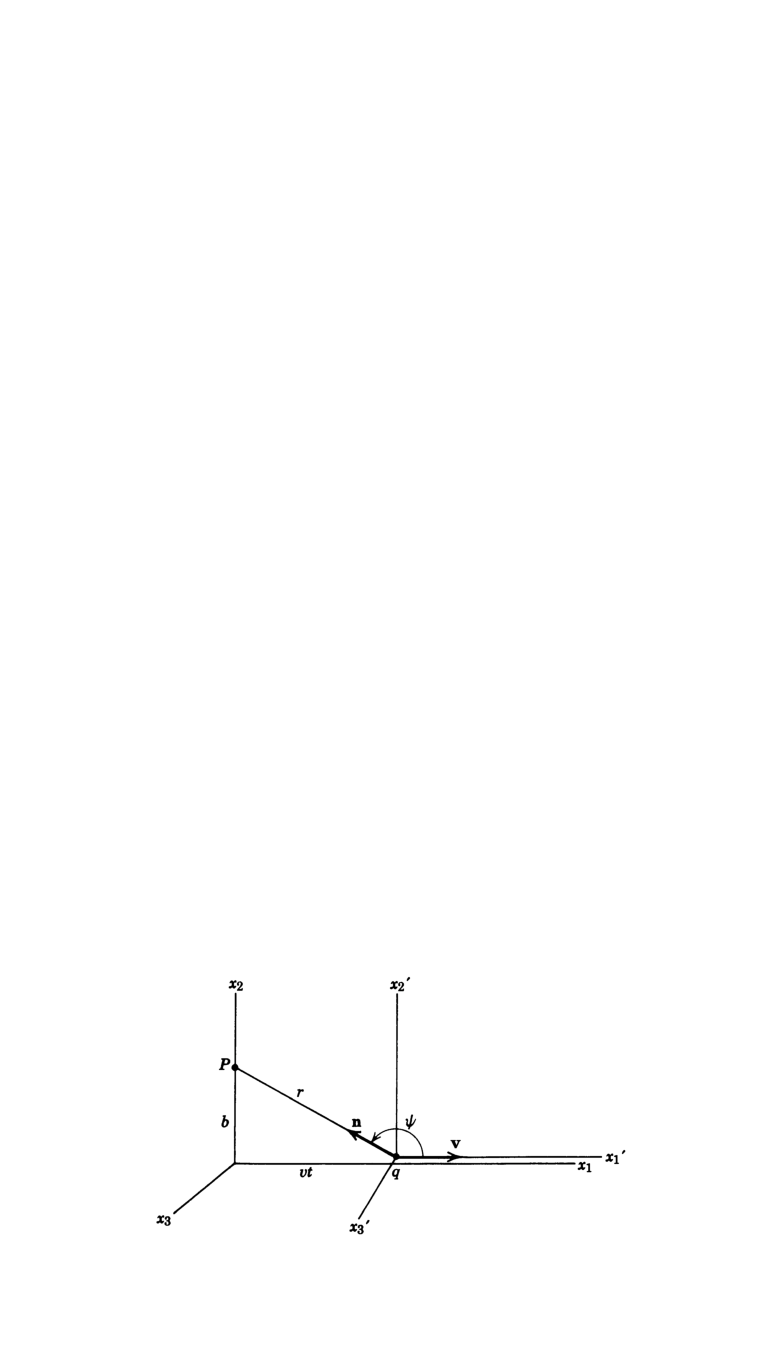
\includegraphics{11-8}
			\caption{(Jackson Fig.~11.8) Particle of charge $q$ moving at constant velocity $\vv$ passes an observation point $P$ at impact parameter $b$.}
			\label{11.8}
		\end{figure}
	\end{minipage}%
	\hspace{0.05\linewidth}%
	\begin{minipage}{0.475\textwidth} \centering
		\begin{figure}[H]
			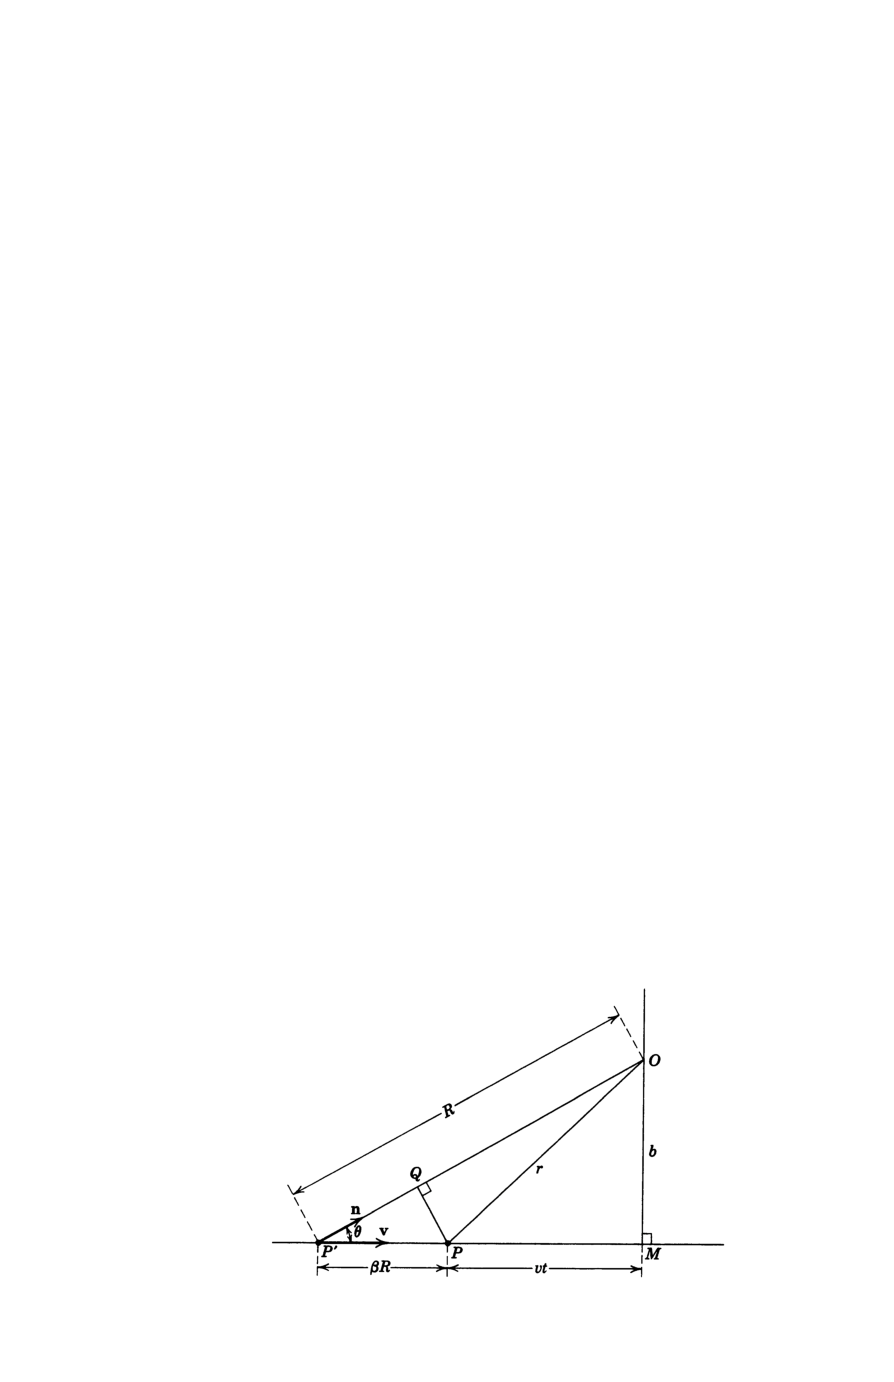
\includegraphics{14-2}
			\caption{(Jackson Fig.~14.2) Present and retarded positions of a charge in uniform motion. \vspace{28pt}}
			\label{14.2}
		\end{figure}
	\end{minipage}
\end{figure}

\sol{
	The {\Lienard}-Wiechert expressions for the fields are given by Jackson~(14.13--14):
	\aln{ \label{LWfields}
		\vB &= [ \nh \cross \vE ]\ret, &
		\vE(\vx, t) &= e \brac{ \frac{\nh - \vbet}{\gam^2 (1 - \vbet \vdot \nh)^3 R^2} }\ret + \frac{e}{c} \brac{ \frac{\nh \cross \{ (\nh - \vbet) \cross \vbetd \}}{(1 - \vbet \vdot \nh)^3 R} }\ret,
	}
	where $\vbet = \vv / c$ with $\vv$ being the particle's velocity, $R$ is the distance from the observation point to the particle's position, and $\nh$ is a unit vector defined by $\vx - \vr(\tau) = R \,\nh$.  Here, $\vr(\tau)$ is the particle's present position and $\tau$ the proper time. 
	
	The expressions for the components of $\vE$ and $\vB$ obtained by a Lorentz transformation are given by Jackson~(11.152):
	\aln{ \label{lorentzfields}
		\Eq &= -\frac{e \gam v t}{(b^2 + \gam^2 v^2 t^2)^{3/2}}, &
		\Ew &= \frac{e \gam b}{(b^2 + \gam^2 v^2 t^2)^{3/2}}, &
		\Ee &= \Bq = \Bw = 0, &
		\Be &= \bet \Ew,
	}
	where the particle is moving in the $\xq$ direction at impact parameter $b$ on the $\xw$ axis, as shown in Fig.~\refeq{11.8}.
	
	For a particle moving with constant velocity in the $\xq$ direction with velocity $v$ as shown in Fig.~\refeq{11.8}, $\vbet = \bet \,\xqh$ and $\vbetd = 0$.  From Jackson~(14.16), note that
	\eq{
		(1 - \vbet \vdot \nh)^2 R^2 = b^2 + v^2 t^2 - \bet^2 b^2
		= \frac{b^2 + \gam^2 v^2 t^2}{\gam^2}
		\qimplies
		(1 - \vbet \vdot \nh)^3 R^2 = \frac{(b^2 + \gam^2 v^2 t^2)^{3/2}}{R \gam^3}.
	}
	This calculation comes from Fig.~\refeq{14.2}, where $O$ is the observation point, $P$ is the present position of the particle, and $P'$ its retarded position.  Also from Fig.~\ref{14.2},
	\eq{
		\nh = \cos\tht \,\xqh + \sin\tht \,\xwh
		= \frac{\bet R - v t}{R} \,\xqh + \frac{b}{R} \,\xwh.
	}
	Making these substitutions in the expression for $\vE(\vx, t)$ in Eq.~\refeq{LWfields},
	\eqn{Efield1}{
		\vE(\vx, t) = e \brac{ \frac{\nh - \vbet}{\gam^2 (1 - \vbet \vdot \nh)^3 R^2} }\ret
		= e \brac{ \frac{(\bet - v t / R - \bet)\,\xqh + (b / R)\,\xwh }{\gam^2 (b^2 + \gam^2 v^2 t^2)^{3/2}} R \gam^3 }\ret
		= e \gam \frac{-v t \,\xqh + b \,\xwh}{(b^2 + \gam^2 v^2 t^2)^{3/2}}.
	}
	For $\vB(\vx, t)$, note that
	\eq{
		\nh \cross \vE \propto \paren{ \frac{\bet R - v t}{R} \,\xqh + \frac{b}{R} \,\xwh } \cross (-v t \,\xqh + b \,\xwh)
		= \paren{ b \frac{\bet R - v t}{R} + \frac{b v t}{R} } \xeh
		= \bet b,
	}
	so
	\eqn{Bfield1}{
		\vB(\vx, t) = e \gam \frac{\bet b \,\xeh}{(b^2 + \gam^2 v^2 t^2)^{3/2}}.
	}
	Writing Eqs.~\refeq{Efield1} and \refeq{Bfield1} in component notation, we find
	\al{
		\Eq &= -\frac{e \gam v t}{(b^2 + \gam^2 v^2 t^2)^{3/2}}, &
		\Ew &= \frac{e \gam b}{(b^2 + \gam^2 v^2 t^2)^{3/2}}, &
		\Ee &= 0, \\
		\Bq &= 0, &
		\Bw &= 0, &
		\Be &= \frac{e \gam \bet b}{(b^2 + \gam^2 v^2 t^2)^{3/2}}
		= \bet \Ew,
	}
	which are identical to Eq.~\refeq{lorentzfields} as was to be shown. \qed
}